\documentclass{standalone}
\usepackage{pgfplots}
\pgfplotsset{compat=1.17}
\usepackage{amsmath}

\begin{document}

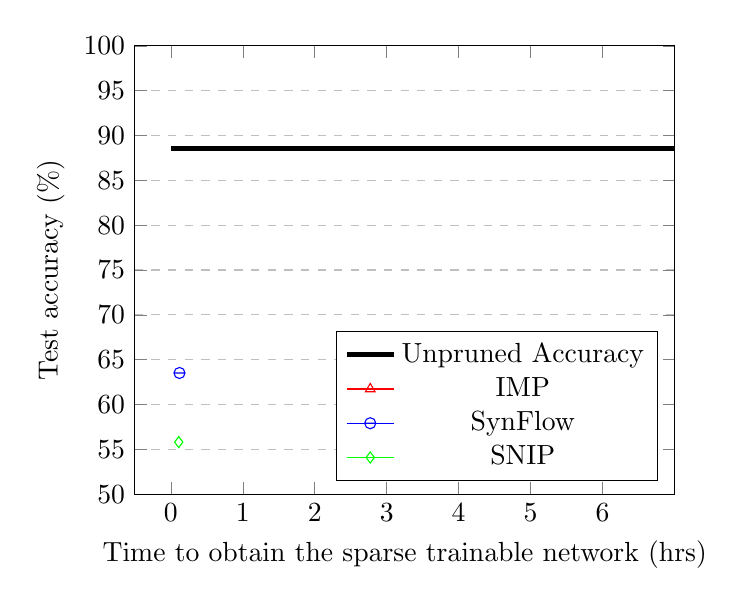
\begin{tikzpicture}
\begin{axis}[
    xlabel={Time to obtain the sparse trainable network (hrs)},
    ylabel={Test accuracy (\%)},
    xmin=-0.5, xmax=7,
    ymin=50, ymax=100,
    xtick={0,1,2,3,4,5,6},
    ytick={50,55,60,65,70,75,80,85,90,95,100},
    legend pos=south east,
    ymajorgrids=true,
    grid style=dashed,
]

% Unpruned Accuracy
\addplot[
    color=black,
    ultra thick,
    ]
    coordinates {
    (0,88.54) (7,88.54)
    };
\addlegendentry{Unpruned Accuracy}

% IMP
\addplot[
    color=red,
    mark=triangle,
    ]
    coordinates {
    (4.0,56.89)
    };
\addlegendentry{IMP}

% SynFlow
\addplot[
    color=blue,
    mark=halfcircle,
    mark options={rotate=180},
    ]
    coordinates {
    (0.12,63.51)
    };
\addlegendentry{SynFlow}

% SNIP
\addplot[
    color=green,
    mark=diamond,
    ]
    coordinates {
    (0.11,55.80)
    };
\addlegendentry{SNIP}

\end{axis}
\end{tikzpicture}

\end{document}